\section{Appendix}
\setlength{\parindent}{0cm}
\textbf{[1] Accuracy score for selection of variables:}
\begin{table}[h]
\caption{Accuracy score for selection [SVM:Gamma=Auto]} % title of Table
\centering % used for centering table
\scalebox{0.8}{
\begin{tabular}{c c c c} % centered columns (4 columns)
\hline\hline %inserts double horizontal lines
Original variables & Selected variables & C value \\ [0.5ex] % inserts table
%heading
\hline % inserts single horizontal line
\\
$0.87$  & $0.85$ & $1$ \\ % inserting body of the table
$0.88$  & $0.85$ & $3$ \\
$0.88$  & $0.85$ & $5$ \\
$0.88$  & $0.84$ & $8$ \\[1ex]
\hline %inserts single line
\end{tabular}}
\end{table}
\\
\par
Produced by the function "ExtraTreesClassifier" by Scikit learn.
\\
\par
\textbf{[2] Extended results for variable analysis:}
\begin{figure}[H]
  \centering
  \subfloat[Minimum imapct for flipped case]{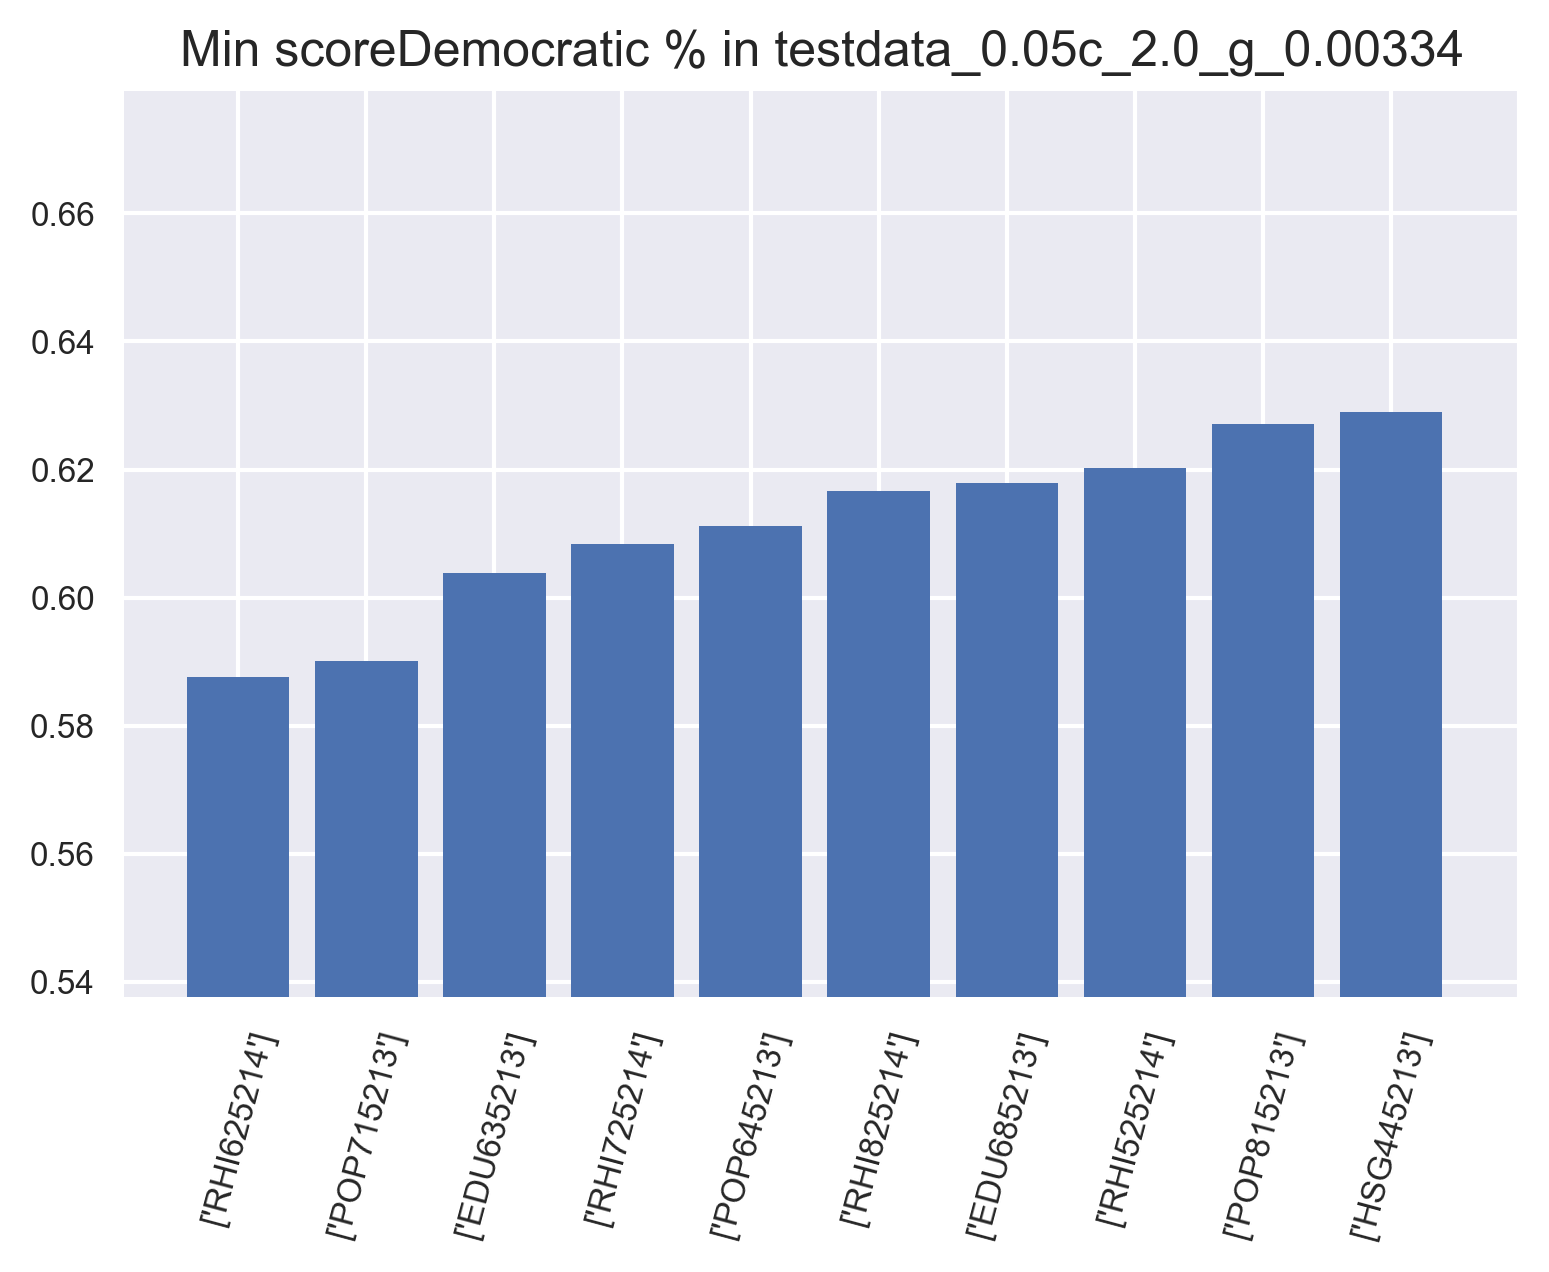
\includegraphics[width=0.5\textwidth]{pictures/results/min_flipp}\label{fig:f3}}
  \hfill
  \subfloat[Maximum imapct for 2016]{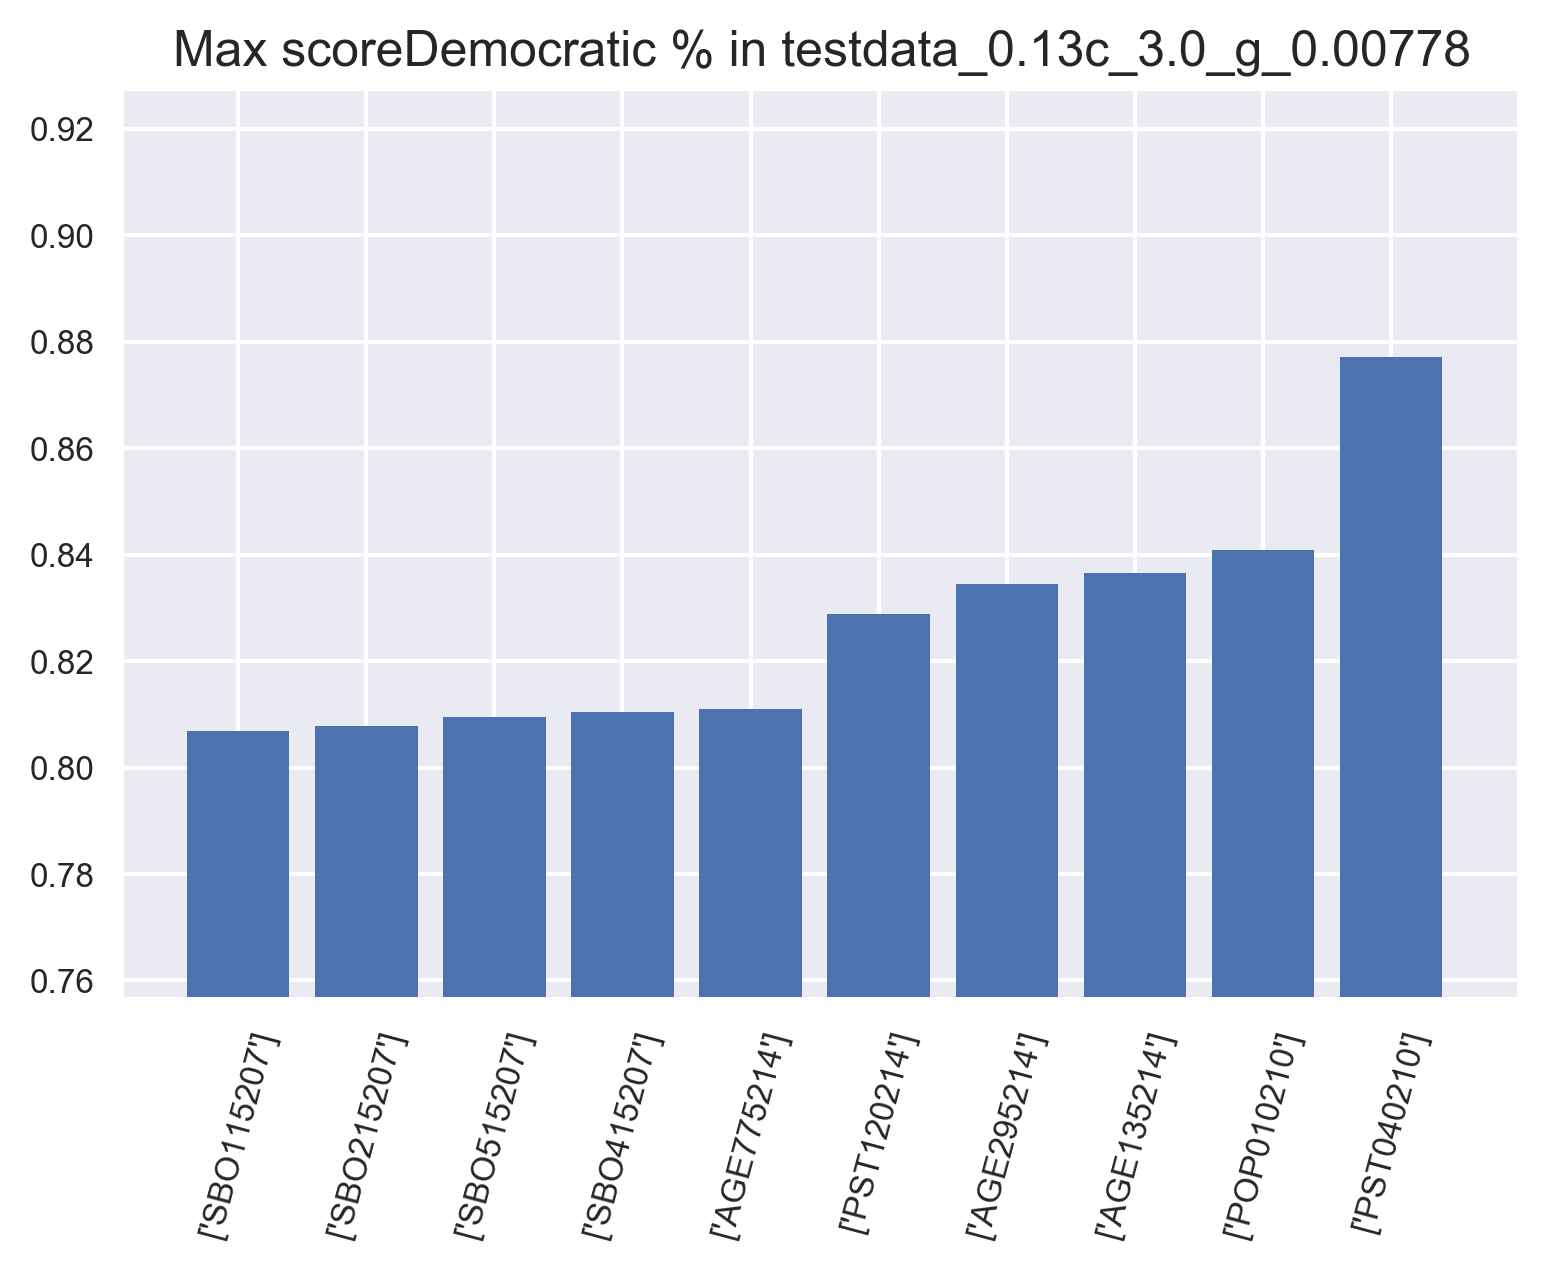
\includegraphics[width=0.5\textwidth]{pictures/results/max_16}\label{fig:f4}}
   \caption{Single variables}
\end{figure}
\begin{figure}[H]
  \centering
  \subfloat[Minimum imapct for 2016]{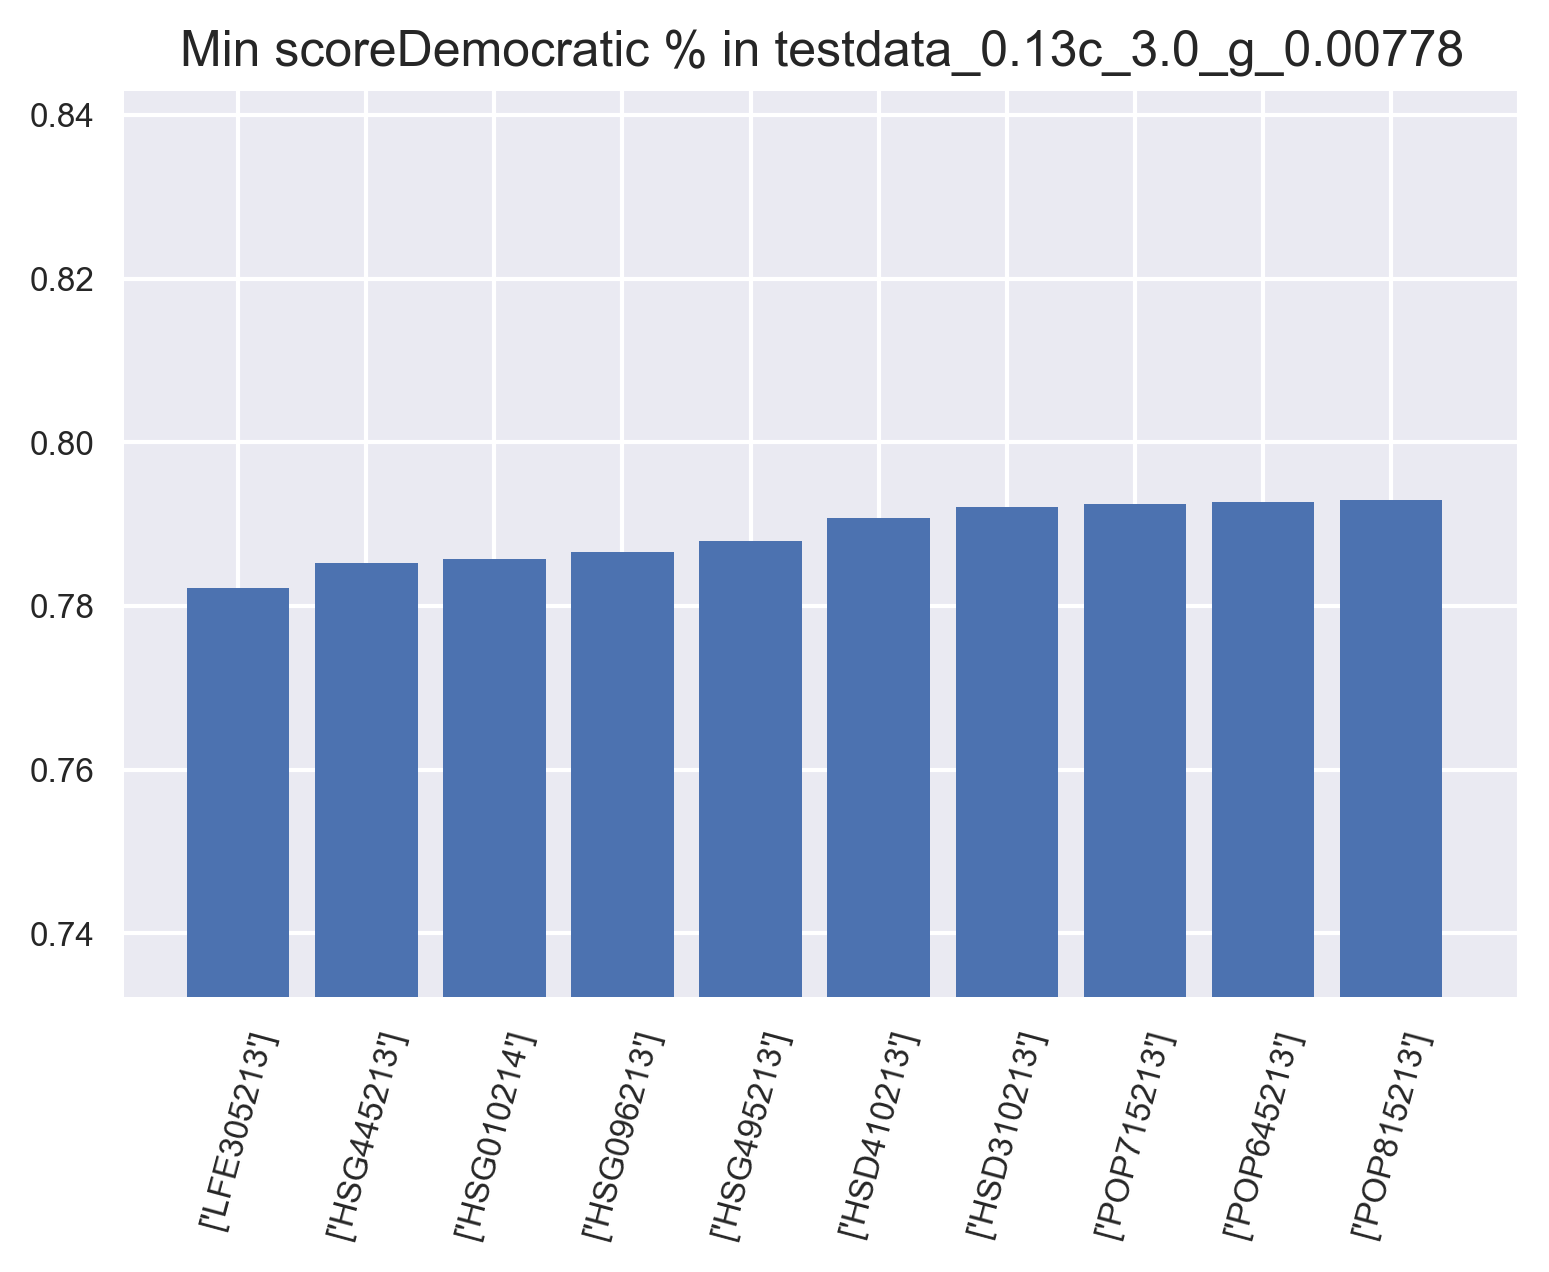
\includegraphics[width=0.5\textwidth]{pictures/results/min_16}\label{fig:f3}}
  \hfill
  \subfloat[Minimum imapct for 2012]{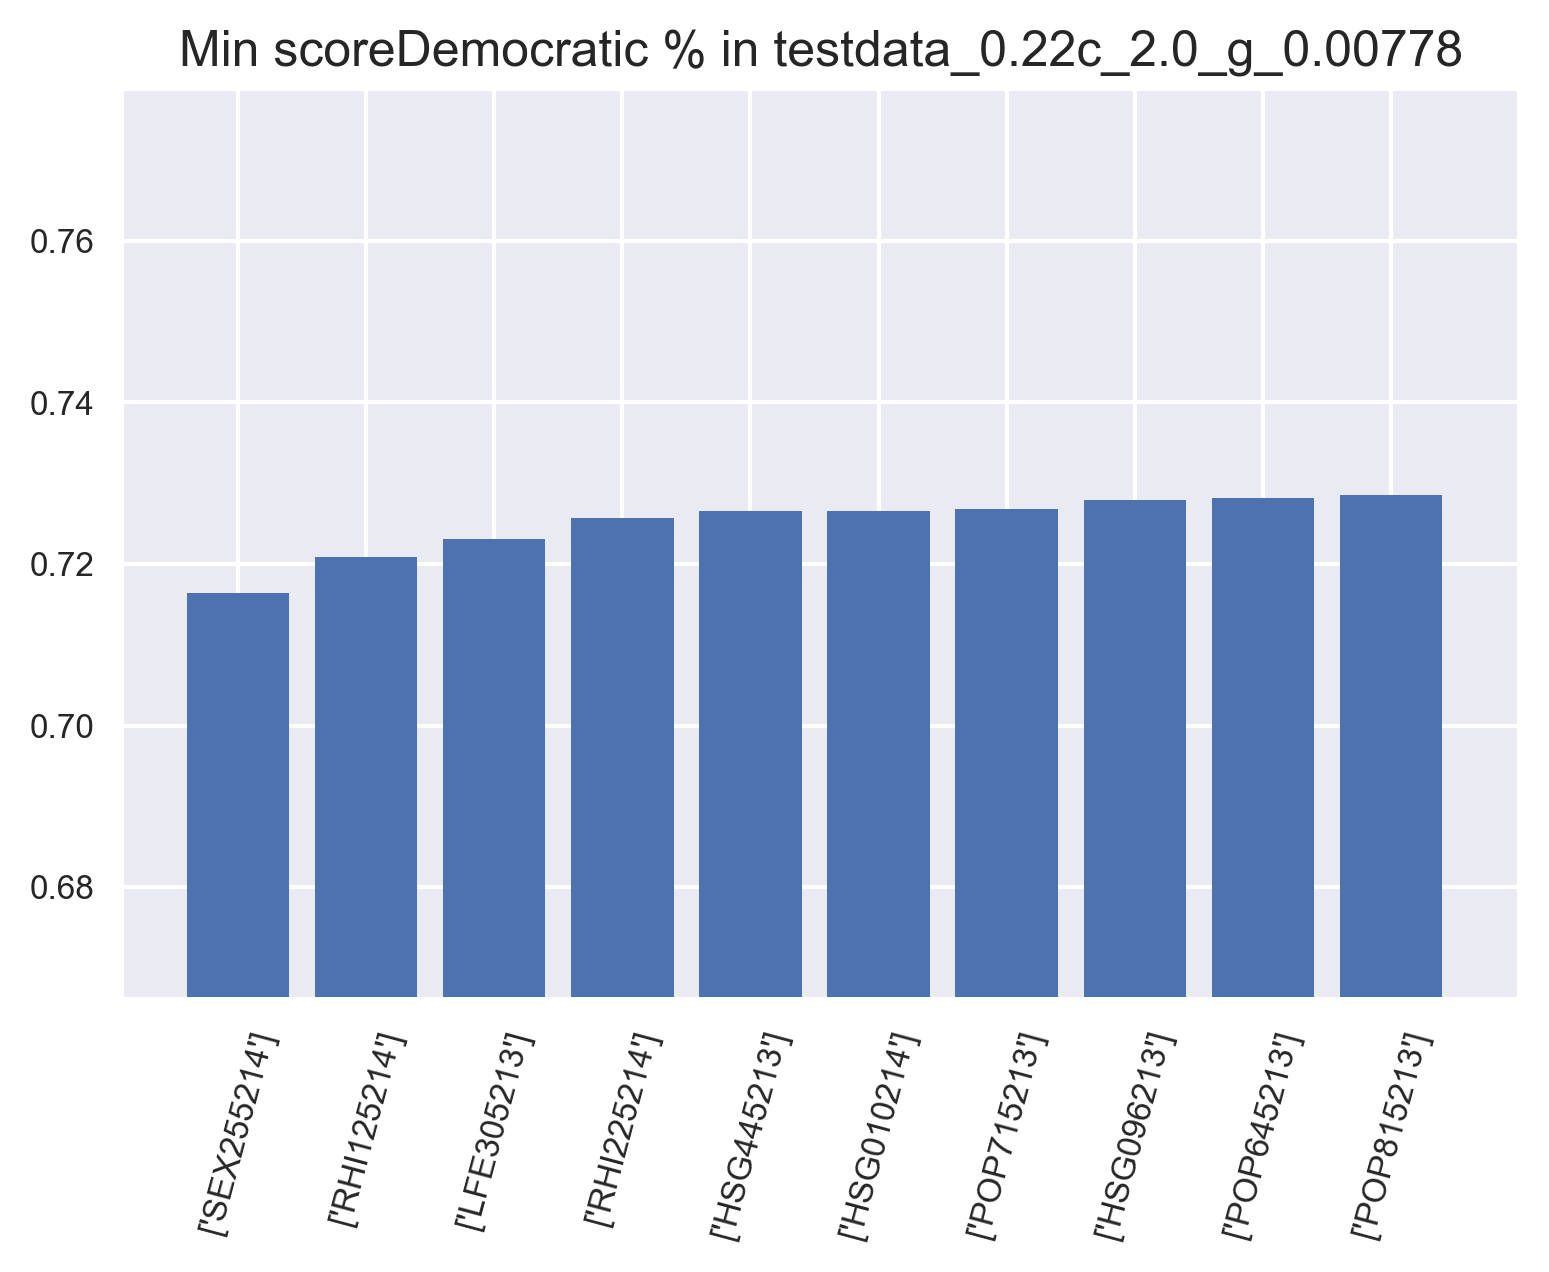
\includegraphics[width=0.5\textwidth]{pictures/results/min_12}\label{fig:f4}}
   \caption{Single variables}
\end{figure}

\textbf{[3] List of variable abbreviations:}\\
PST = Population\\
POP = Population\\
AGE = Age data\\
SEX = Gender data\\
RHI = Ethnicity data\\
EDU = Education data\\
VET = Veterans data\\
LFE = Travel time for work\\
HSG = Housing data\\
INC = Income data\\
PVY = Poverty data\\
BZA = Private non-farm employment\\
NES = Non-employer establishments\\
SBO = Firms owned by different ethnics\\
MAN = Manufactures shipping\\
WTN = Merchant wholesaler sales\\
RTN = Retail sales\\
AFN = Accommodation and food services sales\\
BSP = Building permits\\
LND = Land area\\
\\
\par
All variables can be found at:\\
\url{https://geodacenter.github.io/data-and-lab//county_election_2012_2016-variables/} 
\\
\par

\textbf{[4] List of previous research:}\\
{\scriptsize \url{http://www.ryan-peach.com/school-projects/2017/5/22/describing-the-2016-election-with-machine-learning} By: Ryan Peach}
\newpage
\textbf{[5] Map of misclassifications:}\\
\begin{figure}[H]
\centering
{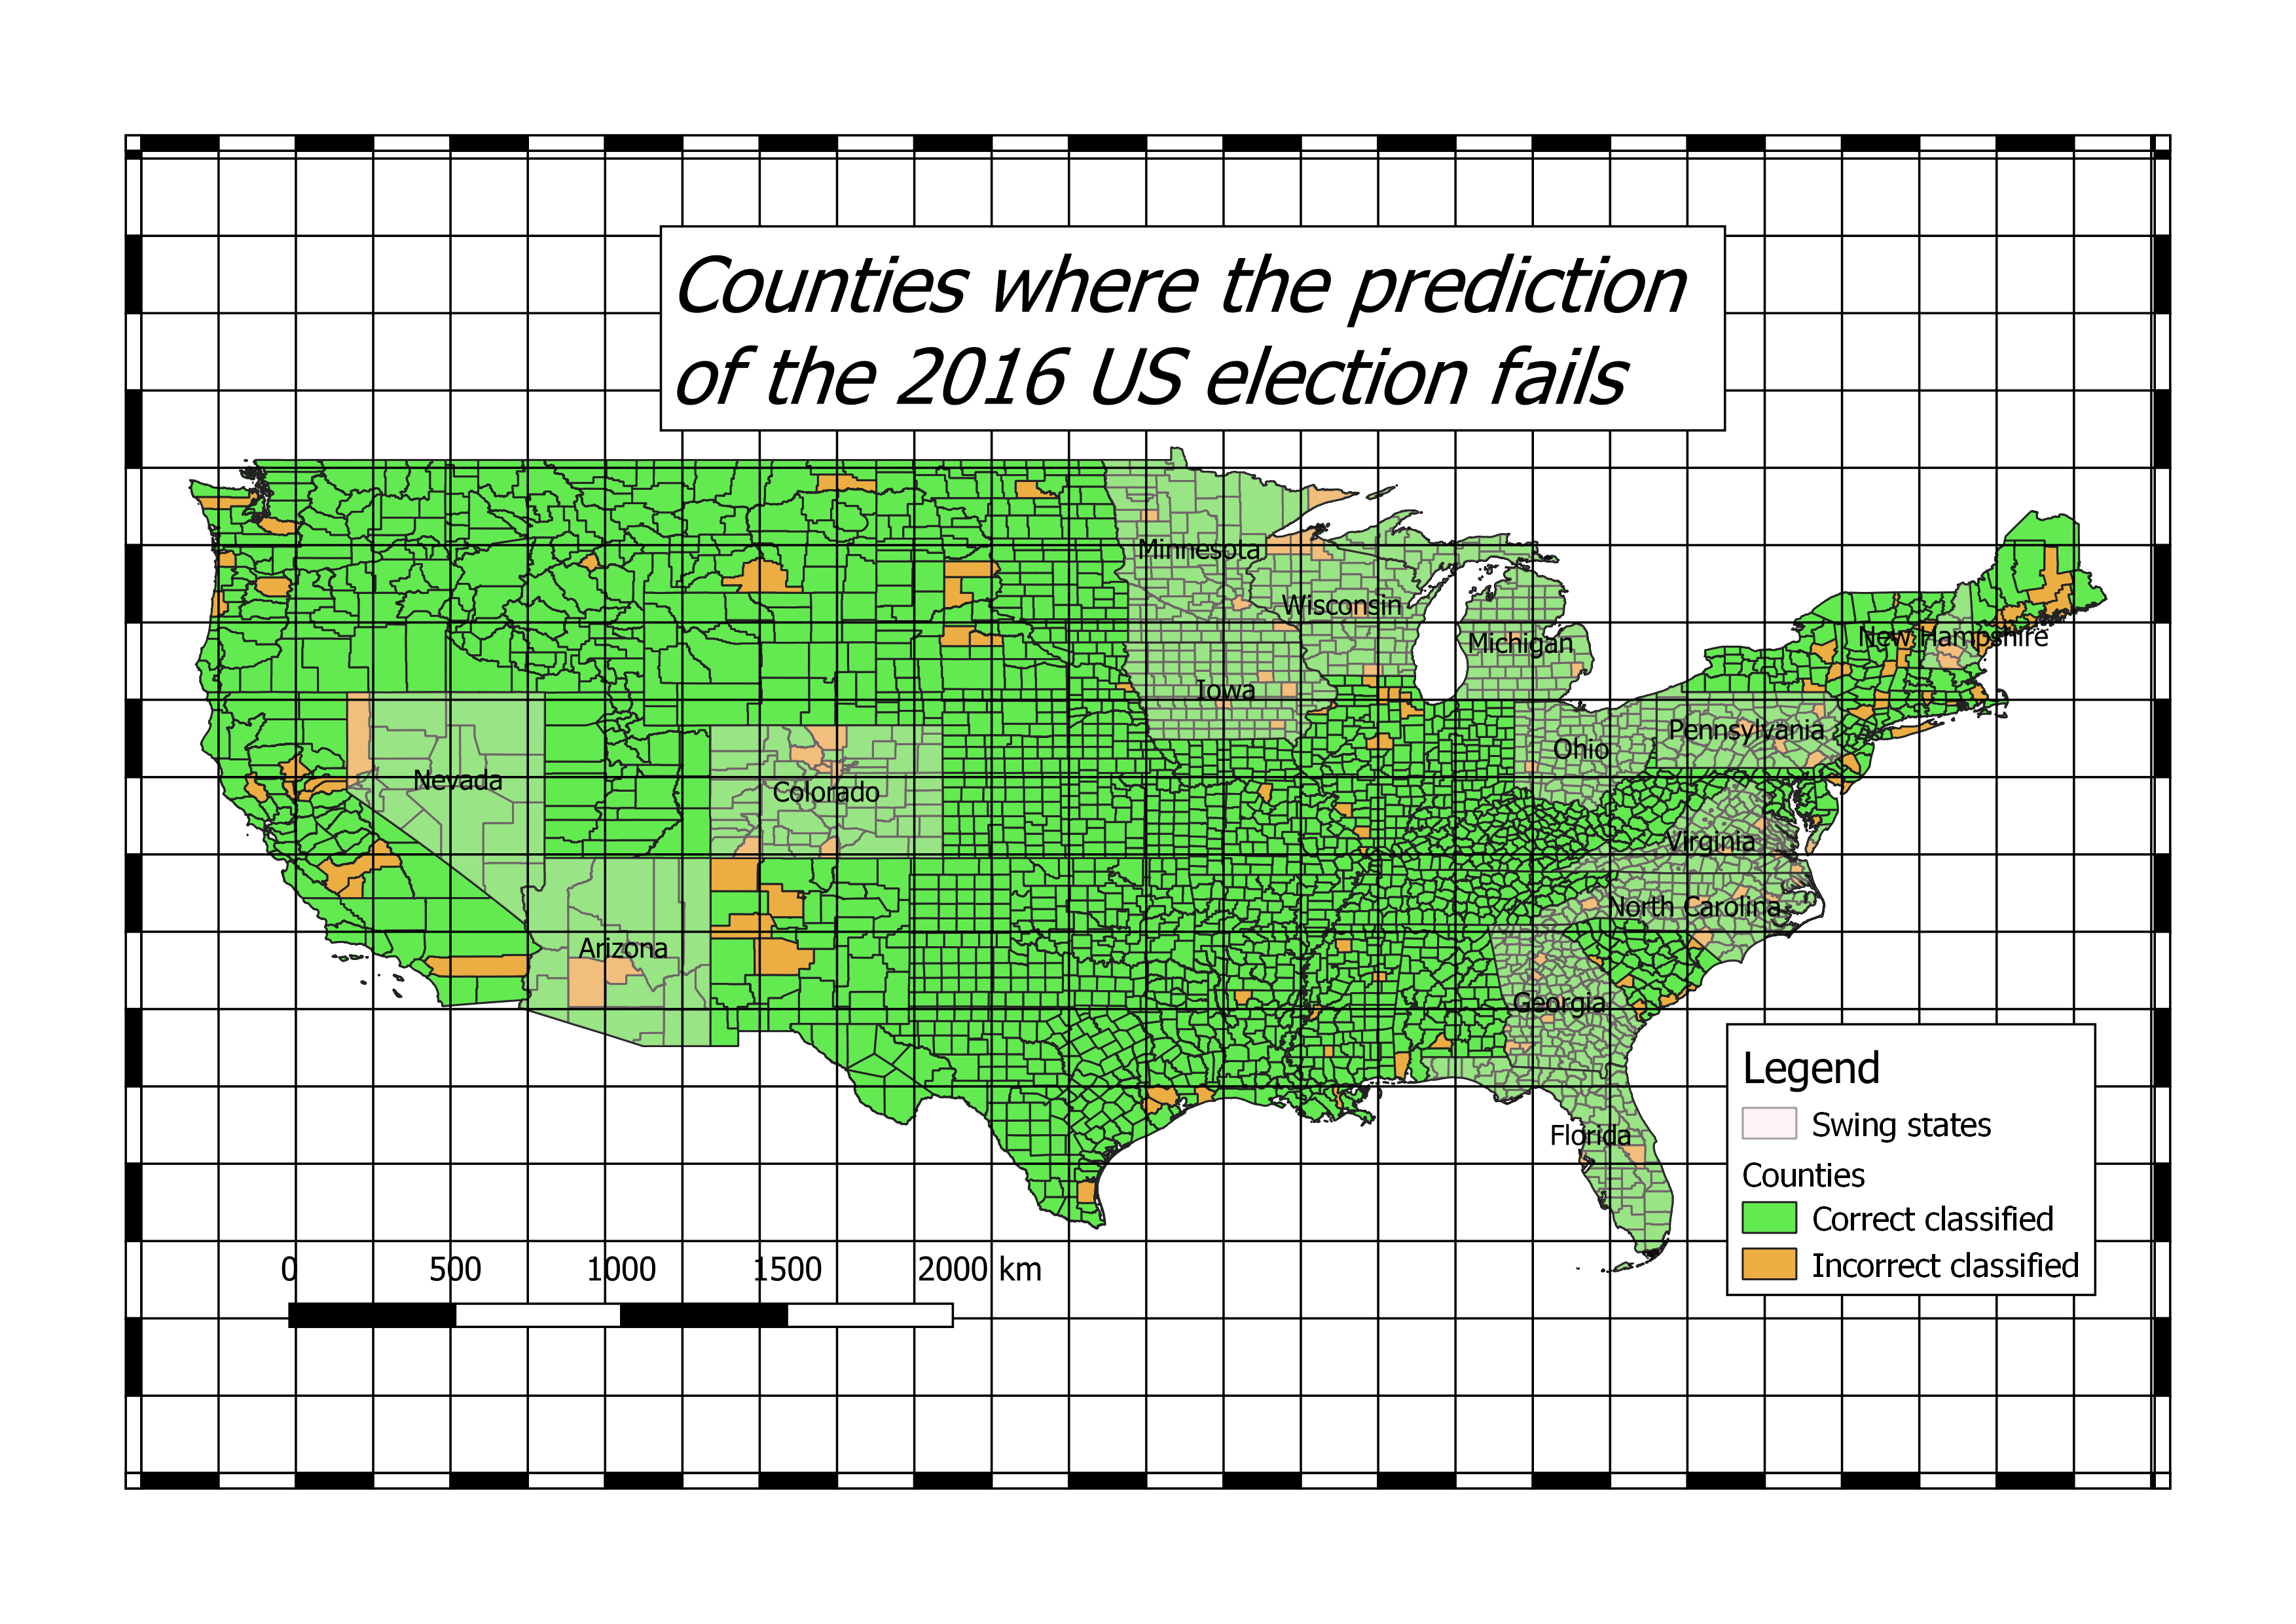
\includegraphics[scale=0.33]{pictures/results/pred}\label{fig:f3}}
\caption{Counties that the SVM kernel could not correctly classify}
\end{figure}

\textbf{[6] Map of flipped counties:}\\
\begin{figure}[H]
\centering
{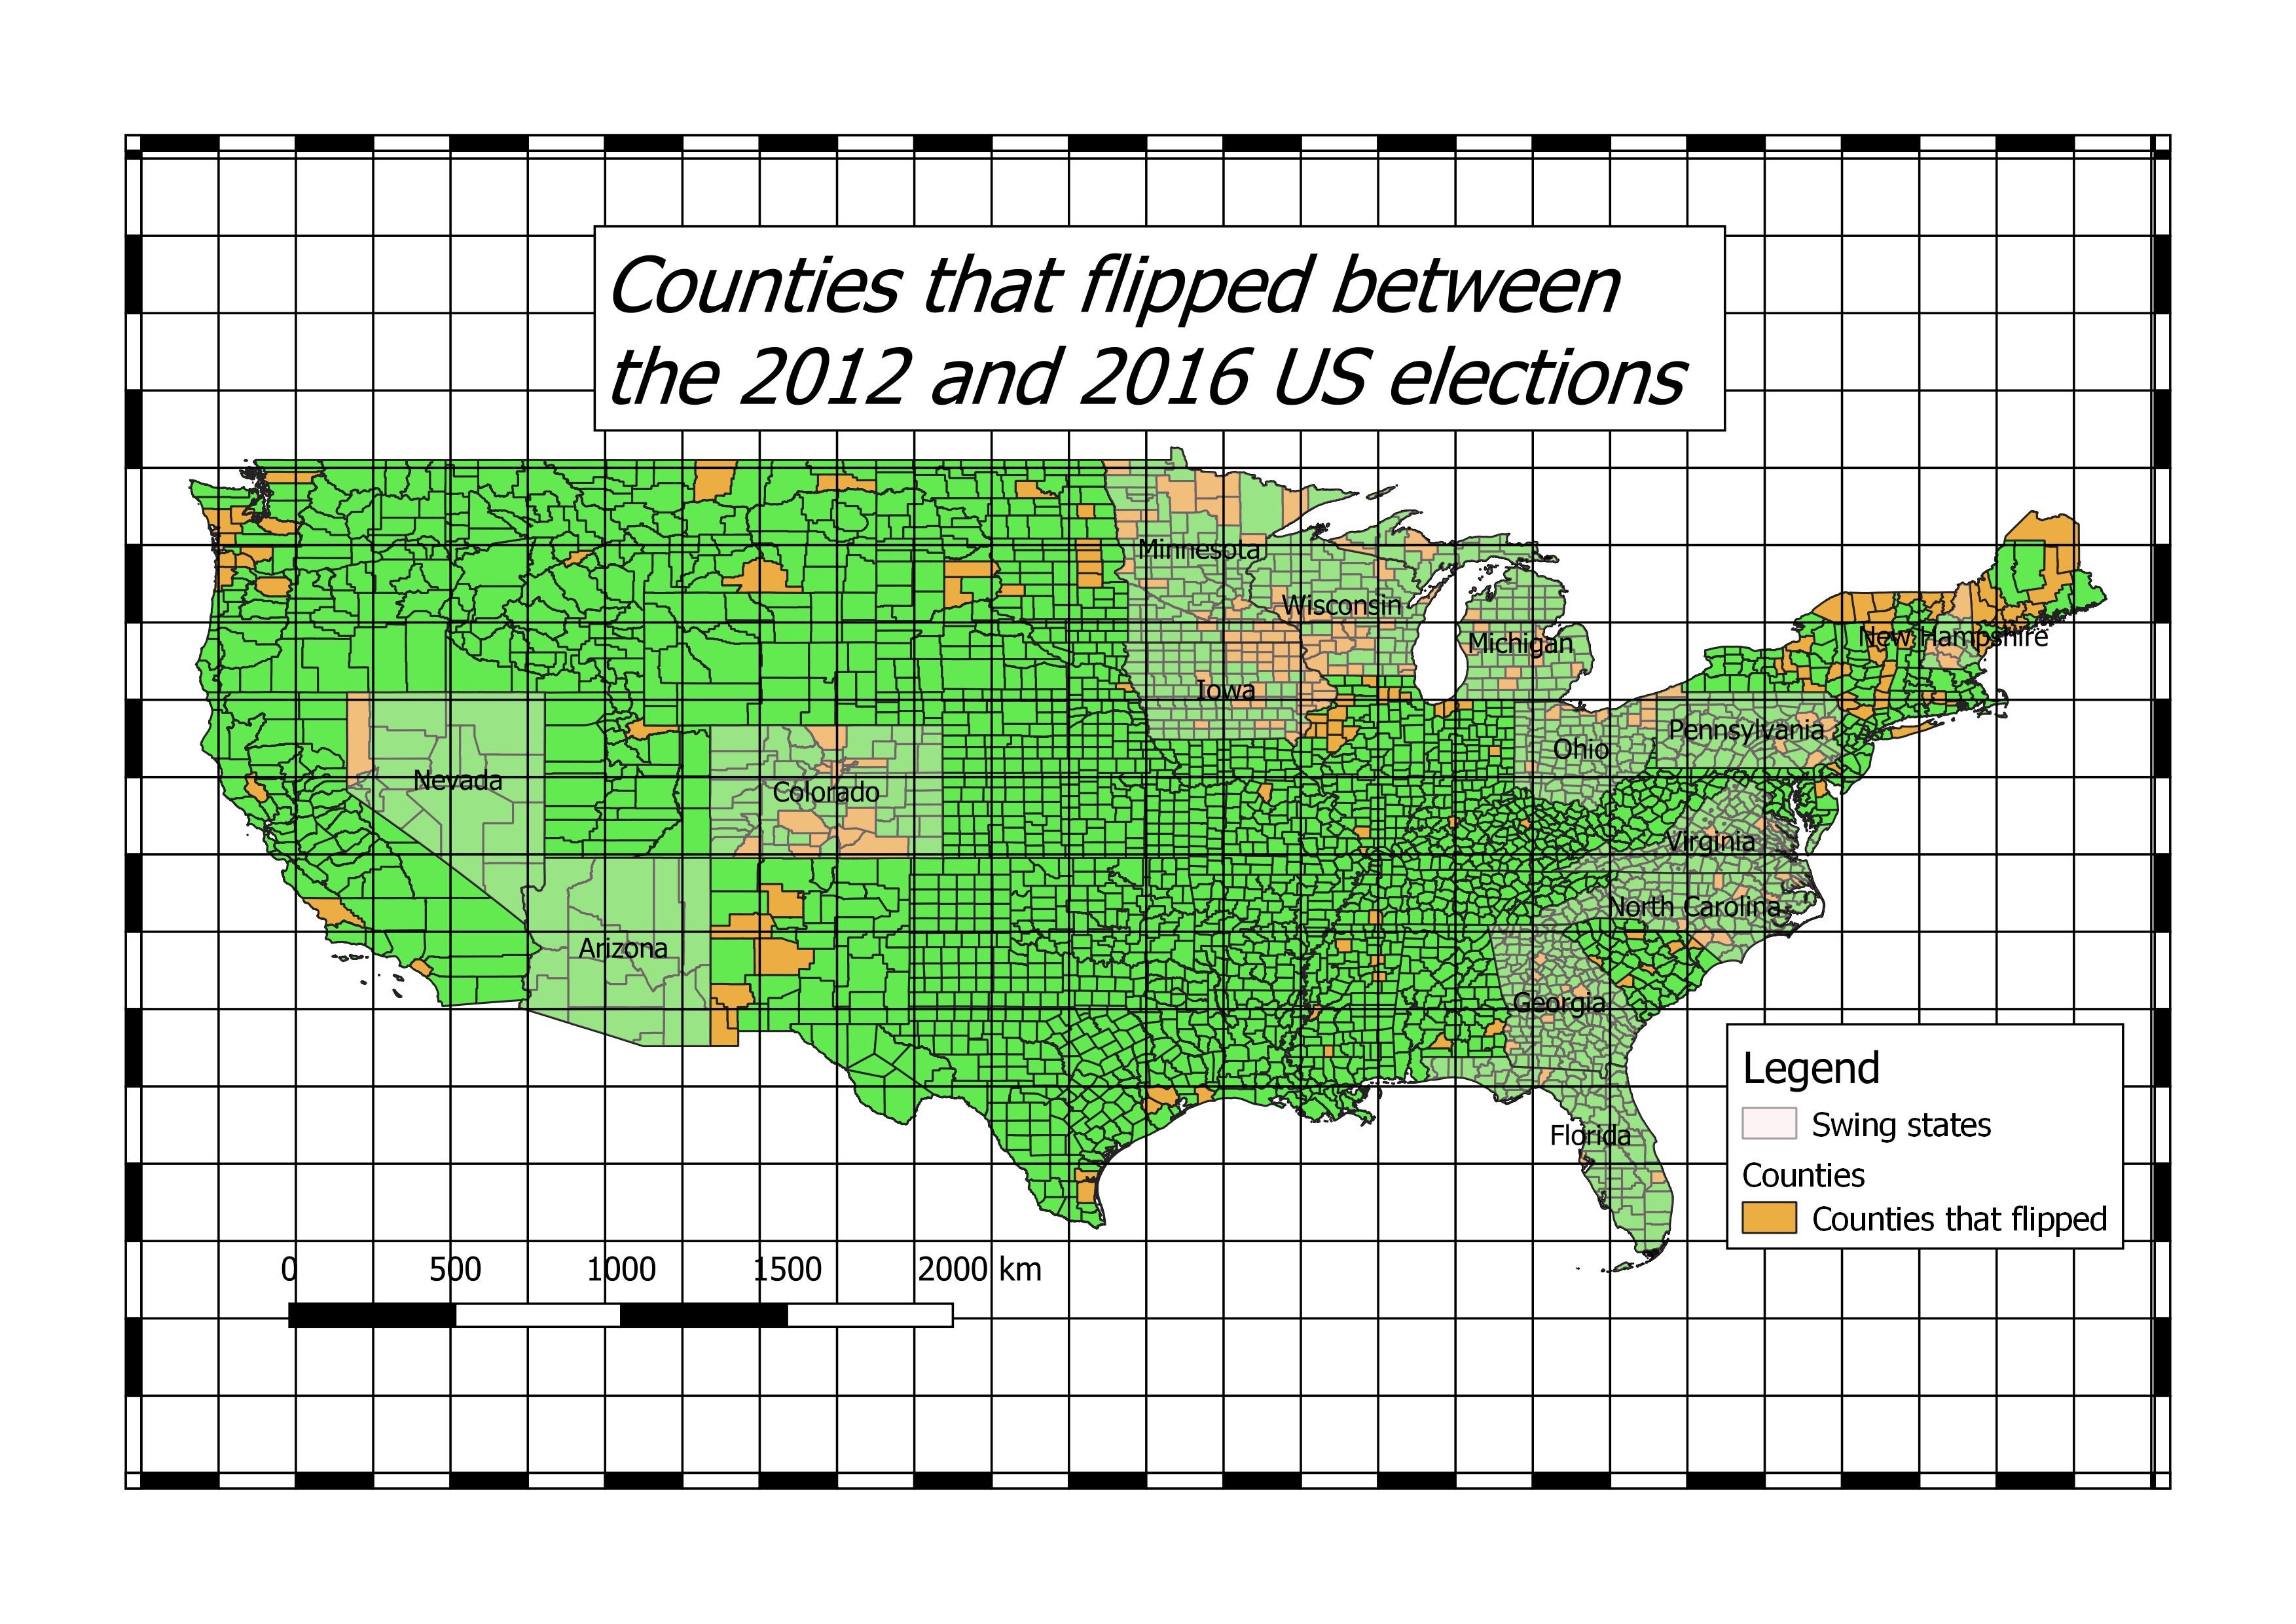
\includegraphics[scale=0.33]{pictures/results/flipps}\label{fig:f3}}
\caption{Map of flipped counties between 2012 and 2016}
\end{figure}

\newpage
\textbf{[7] Cross validation results:}\\

\begin{figure}[H]
\centering
{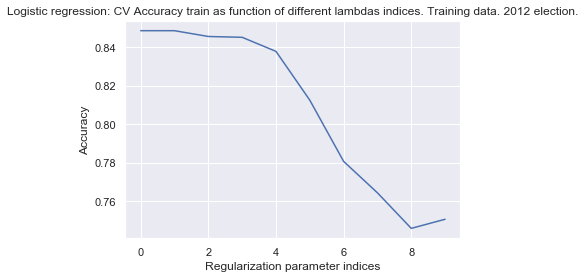
\includegraphics[scale=0.33]{pictures/results/LogReg_Accuracy_train_CV.png}\label{fig:f3}}
\caption{Cross validation results for logistic regression.}
\end{figure}

\begin{figure}[H]
\centering
{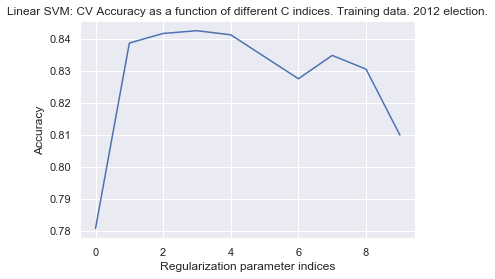
\includegraphics[scale=0.33]{pictures/results/SVML_Accuracy_train_CV.png}\label{fig:f3}}
\caption{Cross validation results for linear SVM.}
\end{figure}

\begin{figure}[H]
\centering
{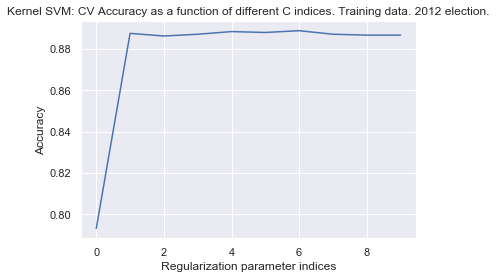
\includegraphics[scale=0.33]{pictures/results/SVMK_Accuracy_train_CV.png}\label{fig:f3}}
\caption{Cross validation results for SVM kernel.}
\end{figure}

\begin{figure}[H]
\centering
{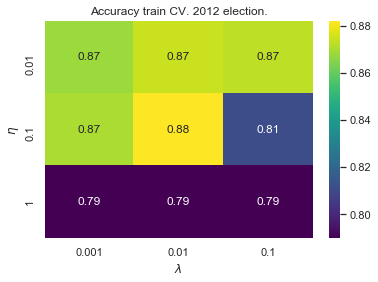
\includegraphics[scale=0.33]{pictures/results/BNN_Accuracy_train_CV.png}\label{fig:f3}}
\caption{Cross validation results for neural network.}
\end{figure}
